%%%%%%%%%% DOCUMENT STUFF %%%%%%%%%%

\documentclass[10.5pt,letterpaper]{article}
\usepackage{mathtools}
\usepackage{amsmath}
\usepackage{amssymb}
\usepackage{datetime}
\usepackage{setspace}
\usepackage{tikz}
\usepackage[margin=1in]{geometry}
\usepackage{courier}
\usepackage{listings}
\usepackage{mips}
\usepackage{graphicx}
\usepackage{enumitem}
\usepackage{pgfplots}

%%%%%%%%%% FORMATTING %%%%%%%%%%

\newdate{date}{15}{05}{2017}
\spacing{1.5}
\date{\displaydate{date}}
\setcounter{secnumdepth}{0}
\newcommand\tab[1][0.5cm]{\hspace*{#1}}
\newcommand*\circled[1]{\tikz[baseline=(char.base)]{
            \node[shape=circle,draw,inner sep=2pt] (char) {#1};}}
\lstset{language=[mips]Assembler}
\usetikzlibrary{arrows,shapes,automata,petri,positioning,calc}

\tikzset{
    place/.style={
        circle,
        thick,
        draw=black,
        fill=gray!50,
        minimum size=6mm,
    },
        state/.style={
        circle,
        thick,
        draw=blue!75,
        fill=blue!20,
        minimum size=6mm,
    },
}


%%%%%%%%%% CONTENT %%%%%%%%%%

%%%%% COVER PAGE %%%%%

\begin{document}
\title{CS 112: Homework 5}
\author{
	Jonathan Woong\\
	804205763\\
	Spring 2017\\
	Discussion 1A}
\maketitle
\pagebreak

%%%%% CONTINUOUS RANDOM VARIABLES %%%%%

\section{Continuous Random Variables}
\begin{enumerate}[label=\textbf{Problem \arabic*.}]
\item There are $N$ machines where $N$ is a large number. Each machine has one of three possible states and changes states (independently) according to a Markov Chain with transition probabilities
\[
\begin{bmatrix}
0.7 & 0.2 & 0.1 \\
0.2 & 0.6 & 0.2 \\
0.1 & 0.4 & 0.5
\end{bmatrix}
\]
What percentage of machines are in each state?
\[\pi = \pi \textbf{P}\]
\[\pi_0 = 0.7\pi_0 + 0.2\pi_1 + 0.1\pi_2\]
\[\pi_1 = 0.2\pi_0 + 0.6\pi_1 + 0.4\pi_2\]
\[\pi_2 = 0.1\pi_0 + 0.2\pi_1 + 0.5\pi_2\]
\[\pi_0 + \pi_1 + \pi_2 = 1\]
\[\pi_0 = 0.35\]
\[\pi_1 = 0.41\]
\[\pi_2 = 0.24\]
\[\boxed{\pi = \begin{bmatrix}0.35 & 0.41 & 0.24\end{bmatrix}}\]
\item Suppose that a node in the computer network is either a host (H), a router (R) or an access point (AP). If the current hop is a host, the next hop will be a host, router, or AP with probabilities 0.5, 0.4, and 0.1, respectively. If the current hop is a router, the next hop will be a host, router or AP with probabilities 0.3, 0.4, and 0.3. If the current hop is an AP, the next hop will be a host, router, or AP with probabilities 0.2, 0.3, 0.5.
	\begin{enumerate}[label=\alph*)]
	\item Find the transition probability matrix \textbf{P}.
	\[\boxed{\textbf{P} = 
	\begin{bmatrix}
	0.5 & 0.4 & 0.1 \\
	0.3 & 0.4 & 0.3 \\
	0.2 & 0.3 & 0.5 
	\end{bmatrix}}\]
	\item Generally, what are the proportions of these three types of nodes?
	\[\pi = \pi \textbf{P}\]
	\[\pi_0 = 0.5\pi_0 + 0.3\pi_1 + 0.2\pi_2\]
	\[\pi_1 = 0.4\pi_0 + 0.4\pi_1 + 0.3\pi_2\]
	\[\pi_2 = 0.1\pi_0 + 0.3\pi_1 + 0.5\pi_2\]
	\[\pi_0 + \pi_1 + \pi_2 = 1\]
	\[\pi_0 = \frac{21}{62}\]
	\[\pi_1 = \frac{23}{62}\]
	\[\pi_2 = \frac{18}{62}\]
	\[\boxed{\pi = \begin{bmatrix}\frac{21}{62} & \frac{23}{62} & \frac{18}{62}\end{bmatrix}}\]
	\end{enumerate}
\item A system is performing a sequence of tasks. Whether or not the current task will successfully be performed depends on the results of the previous two tasks. Suppose that the previous two takes are both successfully performed, then the current task will be successful with probability 0.7; if the last task was successfull, but the one before last one is a failure, then the current one will be successful with probability 0.5; if the last one was a failure but the one before last one was successful, then the current one will be successful with probability 0.4. If both the last one and the one before the last one failed, then the current one will be successful with probability 0.2.
	\begin{enumerate}[label=\alph*)]
	\item Define appropriate states in order to make the above model a Markov Chain.\\
	Let $S$ = success, and $F$ = failure.
		\begin{itemize}
			\item State 0 ($SS$): both success
			\item State 1 ($FS$): success in last, fail one before last
			\item State 2 ($SF$): fail in last, success one before last
			\item State 3 ($FF$): both fail
		\end{itemize}
	\item Find the transition probabilty matrix \textbf{P} for the states defined in part (a).
	\[\boxed{\textbf{P} = \begin{bmatrix}
	0.7 & 0 & 0.3 & 0 \\
	0.5 & 0 & 0.5 & 0 \\
	0 & 0.4 & 0 & 0.6 \\
	0 & 0.2 & 0 & 0.8
	\end{bmatrix}}\]
	\end{enumerate}
\item Suppose that there are two computer vision algorithms for detecting objects. According to the statistics, algorithm $A$ has a correct detection rate of 0.7, and algorithm $B$ has a correct detection rate of 0.6. If the algorithm used this time yields correct detection result, then we will use algorithm $A$ next time; if the algorithm used this time yields incorrect detection result, then we will select algorithm $B$ next time. If the algorithm selected for the first time is equally likely to be algorithm $A$ or $B$, then what is the probability that the algorithm used for the fourth time is algorithm $A$?
\[\textbf{P} = \begin{bmatrix}0.7 & 0.3 \\ 0.6 & 0.4\end{bmatrix}\]
\[\textbf{P}^2 = \begin{bmatrix}0.67 & 0.33 \\ 0.66 & 0.34\end{bmatrix}\]
\[\textbf{P}^3 = \begin{bmatrix}0.667 & 0.333 \\ 0.666 & 0.334\end{bmatrix}\]
\[\boxed{\frac{1}{2}\begin{bmatrix}P_{11}^3 + P_{21}^3\end{bmatrix}=0.6665}\]
\item In a mobile ad hoc network (a network formed by the hosts themselves without the help of infrastructures), three out of every four laptops are connected to a cellphone, while one of every file cellphones is connected to a laptop. What fraction of devices are laptops?
\[\textbf{P} = \begin{bmatrix}0.8 & 0.2 \\ 0.75 & 0.25\end{bmatrix}\]
\[\pi = \begin{bmatrix}\frac{15}{19} & \frac{4}{19}\end{bmatrix}\]
\[\boxed{\frac{4}{19} \text{ are laptops}}\]
\item An instruction for a RISC cpu is either R-type (R), Store/Load (S), or Jump-type (J). If the current instruction is R-type, then the next instruction will be R, S, or J with probabilities 0.5, 0.4, and 0.1, respectively. If the current instruction is Store/Load, then the probabilities for the next instruction to be R, S, or J are 0.3, 0.4, and 0.3, respectively. If the current instruction is Jump-type, then the next instruction will be R, S, or J with probabilities 0.2, 0.3, 0.5, respectively.
	\begin{enumerate}[label=\alph*)]
	\item Draw the state transition diagram.
		\begin{center}
		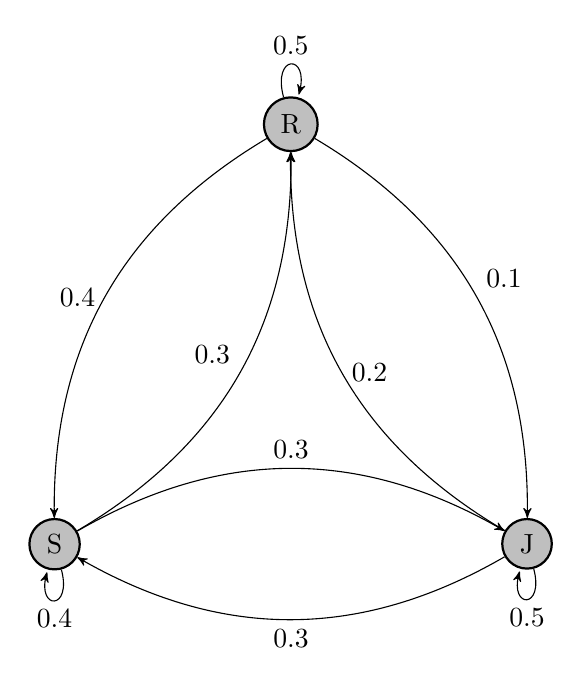
\begin{tikzpicture}[node distance=4cm and 2cm,>=stealth',auto, every place/.style={draw}]
	    \node [place] (R) {R};
	    \coordinate[node distance=3cm,left of=R] (left-R);
	    \coordinate[node distance=3cm,right of=R] (right-R);
	    \node [place] (S) [node distance=5cm,below =of left-R] {S};
	    \node [place] (J) [node distance=5cm,below =of right-R] {J};    
	    \path[->] (R) edge [bend right] node [left] {0.4} (S);
	    \path[->] (R) edge [bend left] node {0.1} (J);
	    \path[->] (R) edge [loop above] node {0.5} (); 
	    \path[->] (S) edge [bend right] node {0.3} (R);
	    \path[->] (S) edge [bend left] node {0.3} (J);
	    \path[->] (S) edge [loop below] node {0.4} ();
	    \path[->] (J) edge [bend left] node [right] {0.2} (R);
	    \path[->] (J) edge [bend left] node {0.3} (S);
	    \path[->] (J) edge [loop below] node {0.5} ();          
	\end{tikzpicture}
	\end{center}
	\item Find the transition probability matrix \textbf{P}.
	\[\boxed{\textbf{P} = 
	\begin{bmatrix}
	0.5 & 0.4 & 0.1 \\
	0.3 & 0.4 & 0.3 \\
	0.2 & 0.3 & 0.5 
	\end{bmatrix}}\]
	\item In the long run, what proportion of instructions are of each type?
	\[\pi = \pi \textbf{P}\]
	\[\pi_0 = 0.5\pi_0 + 0.3\pi_1 + 0.2\pi_2\]
	\[\pi_1 = 0.4\pi_0 + 0.4\pi_1 + 0.3\pi_2\]
	\[\pi_2 = 0.1\pi_0 + 0.3\pi_1 + 0.5\pi_2\]
	\[\pi_0 + \pi_1 + \pi_2 = 1\]
	\[\pi_0 = \frac{21}{62}\]
	\[\pi_1 = \frac{23}{62}\]
	\[\pi_2 = \frac{18}{62}\]
	\[\boxed{\pi = \begin{bmatrix}\frac{21}{62} & \frac{23}{62} & \frac{18}{62}\end{bmatrix}}\]
	\end{enumerate}
\item A workstation tries to transmit frames through Ethernet. Suppose that whether or not collision occurs in the current transmission depends on the result of the last two transmissions the workstation had. That is, suppose that if collisions have occured in both of the past two transmissions, then with probability 0.7 a collision will occur in the current transmission; if a collision occurs in last transmission but not the transmission before the last one, then a collision will occur in the current transmission with probability 0.5; if a collision occured in the transmission before the last one but not the last one, then one will occur in the current transmission with probability 0.4; if there have been no collisions in the past two transmissions, then a collision will occur in the current transmission with probability 0.2.
	\begin{enumerate}[label=\alph*)]
	\item Denote appropriate states in order to make the above model a Markov Chain.\\
	Let $C$ = collision, and $N$ = no collision.
		\begin{itemize}
			\item State 0 (CC): both collide
			\item State 1 (NC): collide in last, no collide one before last
			\item State 2 (CN): no collide in last, collide one before last
			\item State 3 (NN): both don't collide 
		\end{itemize}
	\item Find the transition probability matrix \textbf{P} for the states defined in part (a).
	\[\boxed{\textbf{P} = \begin{bmatrix}
	0.7 & 0 & 0.3 & 0 \\
	0.5 & 0 & 0.5 & 0 \\
	0 & 0.4 & 0 & 0.6 \\
	0 & 0.2 & 0 & 0.8
	\end{bmatrix}}\]
	\item What fraction of frames cause a collision?
	\[\pi = \pi \textbf{P}\]
	\[\pi_0 = 0.7\pi_0 + 0.5\pi_1\]
	\[\pi_1 = 0.4\pi_2 + 0.2\pi_3\]
	\[\pi_2 = 0.3\pi_0 + 0.5\pi_1\]
	\[\pi_3 = 0.6\pi_2 + 0.8\pi_3\]
	\[\pi_0 + \pi_1 + \pi_2 + \pi_3 = 1\]
	\[\pi_0 = \frac{5}{20}\]
	\[\pi_1 = \frac{3}{20}\]
	\[\pi_2 = \frac{3}{20}\]
	\[\pi_3 = \frac{9}{20}\]
	\[\boxed{
		\pi = 
		\begin{bmatrix}
		\frac{5}{20} & 
		\frac{3}{20} & 
		\frac{3}{20} & 
		\frac{9}{20}
		\end{bmatrix}}\]
	\end{enumerate}
\end{enumerate}
\end{document}